
After introducing Large Language Models (LLMs) and Prompt Engineering techniques, we can now outline the working process followed in this research. We will therefore illustrate the methodology adopted at a general level, providing an introductory overview that will be explored in greater depth in the next chapter.
\section{Which is the need?}
The objective of this thesis work stems from the need to provide a methodology to make the answers to questions asked by users of LLM more informative. In particular, in addition to being informative with respect to the question asked, the answers should be able to cover various aspects, including those of a social and legal nature.
To this end, a study was conducted to understand whether Large Language Models are able to correctly express legal and regulatory concepts. The analysis focused on prompt engineering as a tool for extracting from the models the content most relevant to the legal context, assessing whether any shortcomings in the responses are attributable to intrinsic limitations of the model or to the lack of legal information in the training data.
Therefore, the question we have tried to answer is:\\
\\
\textbf{RQ1:}\textit{Do prompt engineering techniques improve the responses generated considering the legal aspects?}\\
\section{Working Process}
Let's now move on to the description of the adopted methodology, analysing the way in which the different steps integrate with each other to guarantee a coherent and structured analysis. The diagram presented offers an overview of the process followed for the evaluation of the responses, outlining the key phases and their contribution to the validity of the analysis.
\begin{figure}[h]
    \centering
    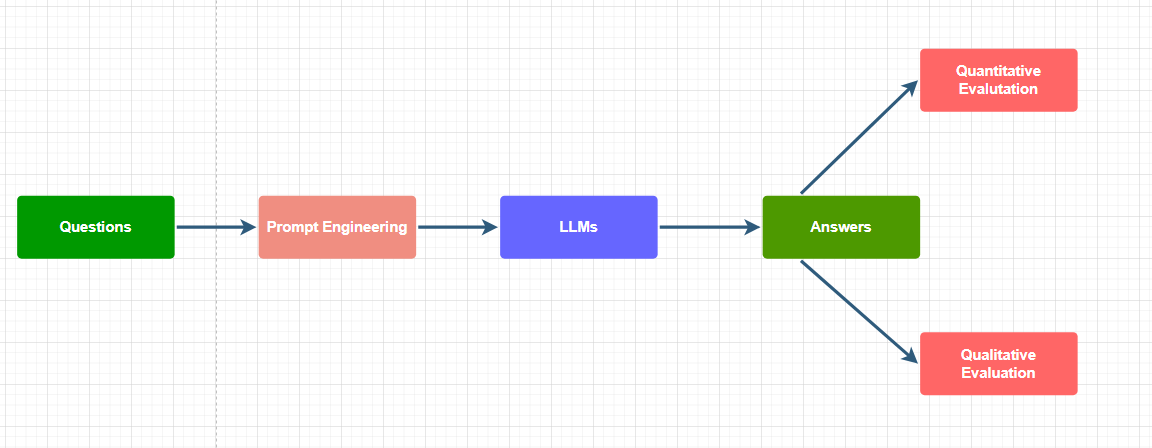
\includegraphics[width=0.7\linewidth]{Figures/Process.png}
    \caption{Development process}
    \label{fig:graph}
\end{figure}
As shown in the graph, the process was divided into four main phases, each of which contributed decisively to the evaluation of the responses.
\begin{enumerate}
    \item \textbf{Selection of questions}:The first phase of the process involved defining the set of questions to be analysed. The selection was made with the support of expert lawyers who, thanks to their knowledge of the sector, contributed to the formulation of questions fully in line with the objectives of the study.
    The selected questions were divided into three main categories:
    \begin{itemize}
        \item \textbf{Legally Neutral}: questions that, at first glance, do not appear to have any legal implications, but which, if analysed in depth, could reveal some.
        \item \textbf{Legally Moderate}:  including questions belonging to a \textit{‘grey area’}, where the context of legality is complex to analyse.
        \item \textbf{Legally Risky}: questions that, in every respect, have explicitly illegal content. 
    \end{itemize}
    Adopting this classification allows us to evaluate the responses of Large Language Models in a wide range of situations, reflecting the different circumstances in which a user might find themselves. 
    \item \textbf{Selection of prompt engineering techniques}: After selecting the questions, an in-depth study was conducted on the different prompt engineering techniques, in order to evaluate their impact on the generation of answers. The analysis of the techniques adopted and their specificities will be illustrated in detail in Chapter \ref{cap:progettazione}.
    \item \textbf{Selection of LLMs}: each of the prompt engineering techniques selected in the previous phase was then applied to each question, using the five LLMs chosen for the analysis. This approach allowed us to compare the answers generated by the different models in relation to the various prompting strategies adopted.
    \item \textbf{Analysis}: After the responses were generated, they were evaluated using two distinct approaches, in order to capture every possible nuance in the evaluations.
    \begin{itemize}
        \item \textbf{Quantitative Analysis}:  In this phase, the distributions of the response classes were compared between the different prompting techniques and the various LLMs, with the aim of evaluating how much the different strategies were able to produce quality responses. The response classes used are:\\
        \begin{itemize}
            \item \textbf{Answer with Warning}:The answer provides information that directly answers the question and, at the same time, indicates any possible risks or legal implications.
            \item \textbf{Answer without Warning}: The answer provides direct information but without warning about possible legal risks.
            \item \textbf{No Answer with Warning}: The answer doesn't directly answer the question, but it warns you about possible legal risks.
            \item \textbf{No Answer without Warning}: The answer is generic and does not provide either a direct answer to the question, or any legal implications.
        \end{itemize}
        In addition, a cross-analysis was carried out between two evaluators, namely myself and an LLM \textit{‘judge’}, in order to measure the agreement on the ability of the answers to inform the user about the legal implications.
        \item \textbf{Qualitative Analisys}:  based on the quantitative analysis, the responses for which the two evaluators did not agree were examined in greater depth, trying to understand which of the two had better grasped the nuances related to the legal implications. This phase allowed for a deeper understanding of the interpretative differences between the evaluators. 
    \end{itemize} 
\end{enumerate}
In the next chapter we will examine in detail the technical choices made, providing an in-depth explanation of the reasons behind each one.